\documentclass[journal]{IEEEtran}
\usepackage{amsmath,amsfonts}
\usepackage{algorithmic}
\usepackage{algorithm}
\usepackage{array}
\usepackage[caption=false,font=normalsize,labelfont=sf,textfont=sf]{subfig}
\usepackage{textcomp}
\usepackage{stfloats}
\usepackage{url}
\usepackage{verbatim}
\usepackage{graphicx}
\usepackage{cite}
\hyphenation{op-tical net-works semi-conduc-tor IEEE-Xplore}
% updated with editorial comments 8/9/2021

\newcommand{\etal}{\textit{et al.}}
\usepackage{multirow}

\begin{document}
	
\title{How to Use \LaTeX\ Draw Beautiful Charts}

\author{XXX, 
	XXX, ~\IEEEmembership{Member, IEEE}, 
	and XXX, ~\IEEEmembership{Senior Member, IEEE}
	
	\IEEEcompsocitemizethanks{\IEEEcompsocthanksitem
		This work was supported in part by the XXX under Grant 123456.
		The authors are with XXX (e-mail: XXX; XXX; XXX).
	}
}

% The paper headers
\markboth{Journal of \LaTeX\ Class Files,~Vol.~14, No.~8, August~2021}%
{XXX \MakeLowercase{\textit{et al.}}: XXX}

% \IEEEpubid{0000--0000/00\$00.00~\copyright~2021 IEEE}
% Remember, if you use this you must call \IEEEpubidadjcol in the second
% column for its text to clear the IEEEpubid mark.

\maketitle


\section{Example}
\begin{table*}[!t]
	\caption{Fingerprint Databases Used in Experiments\label{tab:database}}
	\centering
	\renewcommand{\arraystretch}{1.4}
	\begin{tabular}{| m{1.5cm}<{\centering} | m{3.7cm}<{\centering} | m{3.7cm}<{\centering} | m{3.7cm}<{\centering} | m{3.7cm}<{\centering} |}
		\hline
		\textbf{Database} & FVC2004\_DB1\_A & TDF\_V2\_T & HLD & DPF\_sym\_valid \\
		\hline
		\quad\newline\quad\newline\quad\newline\textbf{Image} 
		& \begin{minipage}[][20mm][c]{.1\textwidth}\centering
			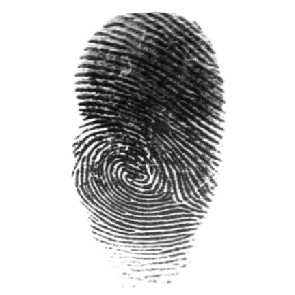
\includegraphics[width=\linewidth]{images/db_ex_1.pdf}
		\end{minipage}
		& \begin{minipage}[][20mm][c]{.1\textwidth}\centering
			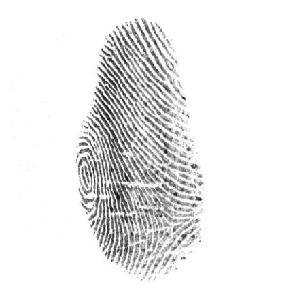
\includegraphics[width=\linewidth]{images/db_ex_2.pdf}
		\end{minipage}
		& \begin{minipage}[][20mm][c]{.1\textwidth}\centering
			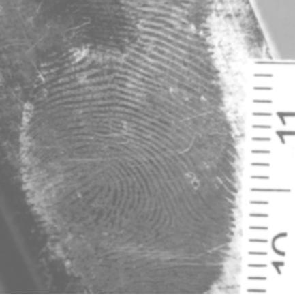
\includegraphics[width=\linewidth]{images/db_ex_3.pdf}
		\end{minipage}
		& \begin{minipage}[][20mm][c]{.1\textwidth}\centering
			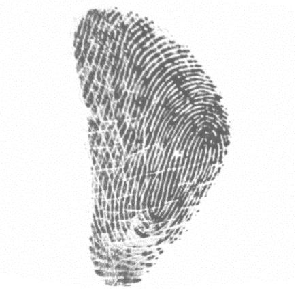
\includegraphics[width=\linewidth]{images/db_ex_4.pdf}
		\end{minipage} \\
		\hline
		\textbf{Sensor} & Optical & Optical & Inking / Optical, Latent & Synthetic \\
		\hline
		\textbf{Description}
		& \multicolumn{1}{m{3.7cm}|}{$800$ fingerprints from $100$ fingers. Most of the poses are frontal. Some fingerprints have large distortion.} 
		& \multicolumn{1}{m{3.7cm}|}{$400$ pairs of normal and mated highly distorted fingerprints from $153$ fingers. Various poses are included.}
		& \multicolumn{1}{m{3.7cm}|}{$1467$ pairs of rolled / plain and mated latent fingerprints from $1467$ fingers in different distortion levels. Various poses are included.}
		& \multicolumn{1}{m{3.7cm}|}{$25,400$ fingerprints generated from $635$ original images of $127$ fingers. Various poses, distortion types and degrees are included.}\\
		\hline
		\textbf{Experiments} 
		& Distoriton estimation accuracy \newline Matching accuracy
		& Distoriton estimation accuracy \newline Matching accuracy
		& Distoriton estimation accuracy \newline Matching accuracy
		& Ablation study\\
		\hline
		\textbf{Genuine Match} 
		& \multicolumn{1}{m{3.7cm}|}{Fingerprints of the same finger are matched each other while symmetric matches are avoided. $2800$ matches in total and $336$ matches in subset.}
		& \multicolumn{1}{m{3.7cm}|}{Each distorted fingerprint is matched with all mated normal fingerprints from the same finger. $2014$ matches in total and $588$ matches in subset.}
		& \multicolumn{1}{m{3.7cm}|}{Each latent fingerprint is mathched with its mated rolled fingerprint. $1467$ matches in total and $765$ matches in subset.}
		& \multicolumn{1}{m{3.7cm}<{\centering}|}{\textbackslash}\\
		\hline
		\textbf{Impostor Match} 
		& \multicolumn{1}{m{3.7cm}|}{First fingerprints of each finger are matched each other while symmetric matches are avoided. $4950$ matches both in total and hard subset.}
		& \multicolumn{1}{m{3.7cm}|}{Each distorted fingerprint is matched with all normal fingerprints from other fingers, $317,305$ matches in total and $59,412$ matches in subset.}
		& \multicolumn{1}{m{3.7cm}|}{Each latent fingerprint is matched with all non-mated rolled fingerprints, $2,150,622$ matches in total and $1,121,490$ matches in subset.}
		& \multicolumn{1}{m{3.7cm}<{\centering}|}{\textbackslash}\\
		\hline
	\end{tabular}
	\renewcommand{\arraystretch}{1}
\end{table*}

\begin{table*}[!t]
	\caption{Distortion Estimation Accuracy of Different Rectification Methods.\label{tab:MRE}}
	\centering
	\renewcommand{\arraystretch}{1.5}
	\begin{tabular}{|m{3.2cm}<{\centering}|m{1.6cm}<{\centering}|m{1.6cm}<{\centering}|m{1.6cm}<{\centering}|m{1.6cm}<{\centering}|m{1.6cm}<{\centering}|m{1.6cm}<{\centering}|}
		\hline
		\multirow{3}{*}{\textbf{Methods}} & \multicolumn{6}{c|}{$\mathbf{MRE\,(\downarrow)}$, $\mathbf{AP\,(\uparrow)}$}\\
		\cline { 2 - 7 } 
		& \multicolumn{2}{m{3.2cm}<{\centering}|}{\textbf{FVC2004\_DB1\_A}\quad\quad\quad\quad}
		& \multicolumn{2}{m{3.2cm}<{\centering}|}{\textbf{TDF\_V2\_T}\quad\quad\quad\quad}  
		& \multicolumn{2}{m{3.2cm}<{\centering}|}{\textbf{HLD}\quad\quad\quad\quad}  \\
		\cline { 2 - 7 }
		& \multicolumn{1}{m{1.6cm}<{\centering}}{\textbf{full}}
		& \multicolumn{1}{m{1.6cm}<{\centering}|}{\textbf{subset}}
		& \multicolumn{1}{m{1.6cm}<{\centering}}{\textbf{full}}
		& \multicolumn{1}{m{1.6cm}<{\centering}|}{\textbf{subset}}  
		& \multicolumn{1}{m{1.6cm}<{\centering}}{\textbf{full}}
		& \multicolumn{1}{m{1.6cm}<{\centering}|}{\textbf{subset}}  \\
		\hline
		\multicolumn{1}{|m{3.2cm}<{\centering}|}{Without Rectification}
		& \multicolumn{1}{m{1.6cm}<{\centering}}{7.66, 32.32}
		& \multicolumn{1}{m{1.6cm}<{\centering}|}{12.39, 23.96}
		& \multicolumn{1}{m{1.6cm}<{\centering}}{12.17, 31.58}
		& \multicolumn{1}{m{1.6cm}<{\centering}|}{12.80, 22.64}  
		& \multicolumn{1}{m{1.6cm}<{\centering}}{13.54, 22.89}
		& \multicolumn{1}{m{1.6cm}<{\centering}|}{15.17, 18.26}  \\
		
		\multicolumn{1}{|m{3.2cm}<{\centering}|}{Gu \etal}
		& \multicolumn{1}{m{1.6cm}<{\centering}}{6.76, 33.59}
		& \multicolumn{1}{m{1.6cm}<{\centering}|}{10.22, 26.97}
		& \multicolumn{1}{m{1.6cm}<{\centering}}{10.53, 33.22}
		& \multicolumn{1}{m{1.6cm}<{\centering}|}{10.81, 24.41}  
		& \multicolumn{1}{m{1.6cm}<{\centering}}{11.66, 24.31}
		& \multicolumn{1}{m{1.6cm}<{\centering}|}{12.64, 19.81}  \\
		
		\multicolumn{1}{|m{3.2cm}<{\centering}|}{Dabouei \etal}
		& \multicolumn{1}{m{1.6cm}<{\centering}}{6.70, 33.54}
		& \multicolumn{1}{m{1.6cm}<{\centering}|}{9.84, 27.16}
		& \multicolumn{1}{m{1.6cm}<{\centering}}{10.12, 33.82}
		& \multicolumn{1}{m{1.6cm}<{\centering}|}{10.53, 25.06}  
		& \multicolumn{1}{m{1.6cm}<{\centering}}{11.37, \underline{\textbf{24.53}}}
		& \multicolumn{1}{m{1.6cm}<{\centering}|}{12.35, 19.92}  \\
		
		\hline
		\multicolumn{1}{|m{3.2cm}<{\centering}|}{Proposed Method}
		& \multicolumn{1}{m{1.6cm}<{\centering}}{\textbf{6.44}, \textbf{33.76}}
		& \multicolumn{1}{m{1.6cm}<{\centering}|}{\textbf{9.46}, \textbf{27.57}}
		& \multicolumn{1}{m{1.6cm}<{\centering}}{\textbf{9.88}, \textbf{34.21}}
		& \multicolumn{1}{m{1.6cm}<{\centering}|}{\textbf{10.10}, \textbf{25.46}}  
		& \multicolumn{1}{m{1.6cm}<{\centering}}{\textbf{11.21}, 24.43}
		& \multicolumn{1}{m{1.6cm}<{\centering}|}{\textbf{12.18}, \textbf{20.06}}  \\
		
		\multicolumn{1}{|m{3.2cm}<{\centering}|}{Proposed Method +O}
		& \multicolumn{1}{m{1.6cm}<{\centering}}{\underline{\textbf{6.34}}, \underline{\textbf{33.77}}}
		& \multicolumn{1}{m{1.6cm}<{\centering}|}{\underline{\textbf{9.10}}, \underline{\textbf{27.82}}}
		& \multicolumn{1}{m{1.6cm}<{\centering}}{\underline{\textbf{9.60}}, \underline{\textbf{34.43}}}
		& \multicolumn{1}{m{1.6cm}<{\centering}|}{\underline{\textbf{9.72}}, \underline{\textbf{25.76}}}  
		& \multicolumn{1}{m{1.6cm}<{\centering}}{\underline{\textbf{11.17}}, \textbf{24.49}}
		& \multicolumn{1}{m{1.6cm}<{\centering}|}{\underline{\textbf{12.04}}, \underline{\textbf{20.28}}}  \\
		\hline
		
		\multicolumn{7}{l}{\emph{Note}: Elements of each column are marked according to their order as \underline{$\textbf{1}^\textbf{st}$} / $\textbf{2}^\textbf{nd}$ / others.}
		
	\end{tabular}
	\renewcommand{\arraystretch}{1}
\end{table*}

\begin{table}[!t]
	\caption{Distortion Estimation Accuracy of the Proposed Network with Different Submodules.\label{tab:ablation}}
	\centering
	\renewcommand{\arraystretch}{1.5}
	\begin{tabular}{|c c c c|c|}
		\hline
		\multicolumn{1}{|m{1.2cm}<{\centering}}{Spatial Pyramid Module} 
		& \multicolumn{1}{m{1.2cm}<{\centering}}{Attention Block} 
		& \multicolumn{1}{m{1.2cm}<{\centering}}{Mask} 
		& \multicolumn{1}{m{1.2cm}<{\centering}|}{Orientation Feature Branch}  
		& \multicolumn{1}{m{1.2cm}<{\centering}|}{$\mathcal{L}_{{\rm dis}}^{\rm{reg}}$}	\\
		\hline
		-			&-			&-			&-			& 109.6\\ 
		$\surd$ 	&- 			&- 			&- 			& 80.7\\
		$\surd$ 	&$\surd$	&- 			&- 			& 77.1\\
		$\surd$ 	&$\surd$	&$\surd$	&- 			& 75.1\\ \hline
		$\surd$ 	&$\surd$	&$\surd$	&$\surd$	& 69.6\\
		\hline
	\end{tabular}
	\renewcommand{\arraystretch}{1}
\end{table}

\begin{table}[!t]
	\caption{Distortion Estimation Accuracy of the Proposed Network with Different Preprocessing(enhancement, binarization, or thinning) and Training Stratigies(single-stage or two-stage).\label{tab:ablation_strategies}}
	\centering
	\renewcommand{\arraystretch}{1.5}
	\begin{tabular}{|c | c c c c|}
		\hline
		\multicolumn{1}{|m{0.7cm}<{\centering}|}{} 
		& \multicolumn{1}{m{1.4cm}<{\centering}}{enhancement \& single-stage} 
		& \multicolumn{1}{m{1.4cm}<{\centering}}{binarization \& single-stage} 
		& \multicolumn{1}{m{1.4cm}<{\centering}}{thinning \quad\& single-stage} 
		& \multicolumn{1}{m{1.4cm}<{\centering}|}{thinning \quad\& \quad two-stage}\\
		\hline
		$\mathcal{L}_{{\rm dis}}^{\rm{reg}}$ & 	72.8 & 71.4	& 69.6	& 78.2 \\ 
		\hline
	\end{tabular}
	\renewcommand{\arraystretch}{1}
\end{table}

\begin{table}[h]
	\caption{Model Size and Efficiency of Different Rectification Methods for Processing a $512\times512$ Distorted Fingerprint in TDF\_V2\_T.\label{tab:cost}}
	\centering
	\renewcommand{\arraystretch}{1.5}
	\begin{tabular}{|l|c|c|}
		\hline
		Methods                      		& Params (M) & Time (s) \\
		\hline
		Gu \etal		& 112.5	& 3.85	\\
		Dabouei \etal 	& 63.0	& 0.39	\\
		\hline
		Proposed		& 11.4	& 0.36	\\
		Proposed +O                               	&  45.0 &  0.41 \\
		\hline
	\end{tabular}
	\renewcommand{\arraystretch}{1}
\end{table}

\end{document}


